\chapter{Risk Assessment}

	The risk assesment table is our base criteria for total risk assessment. The table tells 
	the risk of different combinations of consequence and probability. The consequence and 
	probability is ranked High, Medium and Low. 

		\begin{figure}[H]
			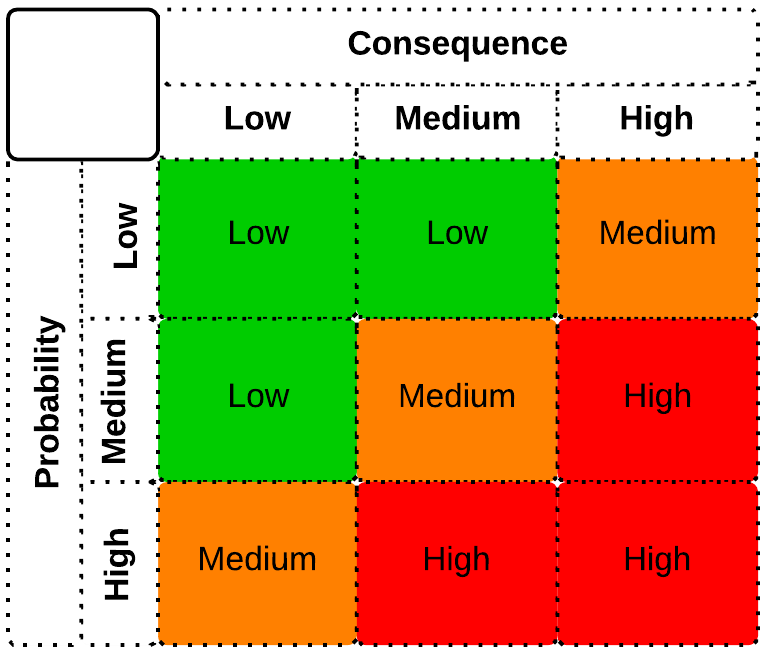
\includegraphics[scale=0.3]{pics/risk.png}
		\end{figure}

	In the following tables we have performed a risk identification and a risk assessment for 
	each separate use case. In the risk identification we have evaluated each function and 
	considered what may go wrong. In addition we have evaluated where in the source code the 
	error may occur. For each risk assessment, we have rated both the probability (Prob.) and consequence (Cons.) for each case, which is the basis for the total risk (Tot.) fetched from the risk assessment table.

	\clearpage


	\begin{landscape}

	\section{Scenario 1}
			\begin{longtable}{ c | p{5cm} | p{5cm} | p{5cm} | c | c | c}
				\hline
				{\bf ID} & {\bf Function} & {\bf Failure mode} & {\bf Code involved} & 
				{\bf Cons.} & {\bf Prob.} & {\bf Tot.} \\ \hline
				1.1 
				& CM enters the new SW component to the system and uploads it to the SW archive
				& CM enters invalid component & FactoryProjectPane, FactoryProject
				& High & Med & High \\ \hline
				1.2 
				& CM adds the new actionscript and uploads it to the Action DB
				& CM enters invalid actionscript
				& FactoryProjectPane, FactoryProject 
				& High & Med & High \\ \hline
		\end{longtable}	

	\section{Scenario 2}

			\begin{longtable}{ c | p{5cm} | p{5cm} | p{5cm} | c | c | c}
				\hline
				{\bf ID} & {\bf Function} & {\bf Failure mode} & {\bf Code involved} & 
				{\bf Cons.} & {\bf Prob.} & {\bf Tot.} \\ \hline
				2.1 
				& CM adds new software to the archive
				& The software already exist. 
				& FactoryProjectPanel, FactoryProject, FactoryDBStorage, SoftwarePanel, Software
				& Low & Low & Low \\ \hline
				2.2 
				& CM update actionscript database
				& Invalid actionscript
				& FactoryDBStorage, CreateFactoryDB
				& High & Med & High \\ \hline
				2.3
				& List of vehicles is send to all registered garage.
				& The garage do not receive the list.
				& FactoryProjectPanel, RecallPanell
				& High & Med & High \\ \hline
				2.4
				& Garage employee identifies relevant car owners.
				& The car has no registered owner
				& ProjectPanel, RecallPanel, PersonPanel, PersonListModel
				& Med & Low & Low \\ \hline
				2.5
				& System sends email to all relevant car owners.
				& Email is not sendt, Sendt email is not received
				& ProjectPanel, RecallPanel, PersonPanel
				& Med & Med & Med \\ \hline
			
		\end{longtable}

	\section{Scenario 3}

		\begin{table}[H]
			\begin{tabular}{ c | p{5cm} | p{5cm} | p{5cm} | c | c | c}
				\hline
				{\bf ID} & {\bf Function} & {\bf Failure mode} & {\bf Code involved} & 
				{\bf Cons.} & {\bf Prob.} & {\bf Tot.} \\ \hline
				3.1 
				& GP identifies the vehicle serial number
				based on the RO's name.  
				& No match on the RO's name in the databse
				& ProjectPanel, SearchPersonAction 
				& Low & Med & Med \\ \hline
				3.2
				& GP downloads the latest version of software
				from the software archive 
				& Could not find the lastest version of software
				in the software archive.
				& ProjectPanel, VehiclePanel, Vehicle, VehicleDBStorage, GUIConnect, garageConnection
				& Med & Low & Low \\ \hline
				3.3 
				& GP updates the vehicles master computer with
				the latest version of software from the Software
				archive 
				& The vehicle is already updated with the latest
				software version.
				& ProjectPanel, Connection, GUIConnect, 
				VehiclePanel, Vehicle
				& Low & Low & Low \\ \hline
				3.4 
				& GP updates the vehicles configuration info 
				in the vehicle DB. 
				& The configuration info was not updated.
				& ProjectPanel, VehiclePanel, 
				Vehicle
				& Med & Med & Med \\ \hline
			\end{tabular}
		\end{table}


	\section{Scenario 4}

		\begin{table}[H]
			\begin{tabular}{ c | p{5cm} | p{5cm} | p{5cm} | c | c | c}
				\hline
				{\bf ID} & {\bf Function} & {\bf Failure mode} & {\bf Code involved} & 
				{\bf Cons.} & {\bf Prob.} & {\bf Tot.} \\ \hline
				4.1
				& CM adds a new actionscript to the action database
				& CM adds a invalid action script
				& FactoryProjectPanel, EcuVehPanel, Ecu, Software, SimpleEcu, EcuDbStorage
				SoftwareDbStorage
				& High & Med & High \\ \hline
				4.2
				& CM adds the new serie of vehicle to the vehicle database
				& Parameters given when adding the new series is not valid
				& FactoryProjectPanel, NewVehiclePanel, Vehicle, VehicleDBStorage
				& Med & Low & Low \\ \hline
				4.3
				& FP adds a new vehicle to the vehicle production series in the vehicle database
				& Parameters given when adding the new vehicle is not valid
				& FactoryProjectPanel, NewVehiclePanel, Vehicle, VehicleDBStorage
				& Low & Med & Low \\ \hline

			\end{tabular}
		\end{table}


\end{landscape}